\documentclass[10pt,letterpaper]{article}
\usepackage[top=1in,bottom=1in,left=1in,right=1in]{geometry}
\usepackage{datetime}
\usepackage{natbib}      % http://merkel.zoneo.net/Latex/natbib.php
\usepackage{palatino}
\usepackage{verbatim}
\usepackage[normalem]{ulem}
\bibpunct{(}{)}{;}{a}{,}{,}

\usepackage{enumitem}
\usepackage{array}

\usepackage{chngpage}
\usepackage{stmaryrd}
\usepackage{amssymb}
\usepackage{amsmath}
\usepackage{graphicx}
\usepackage{lscape}
\usepackage{subfigure}
\usepackage[usenames,dvipsnames]{color}
\definecolor{myblue}{rgb}{0,0.1,0.6}
\definecolor{mygreen}{rgb}{0,0.3,0.1}
\usepackage[colorlinks=true,linkcolor=black,citecolor=mygreen,urlcolor=myblue]{hyperref}

\newcommand{\bocomment}[1]{\textcolor{Bittersweet}{BO says: #1}}

\newcommand{\ignore}[1]{}
\newcommand{\transpose}{^\mathsf{T}}
\newcommand{\inner}[1]{\langle #1 \rangle} 
\newcommand{\smallsec}[1]{\noindent \textbf{#1\ }}
\newcommand{\cmd}[1] {{\color{blue}\texttt{#1}}}

\newcommand{\solution}[1]{{\color{myblue} \emph{[Solution:} 

#1 

\emph{End solution]}}}
\newcommand{\solutionnote}[1]{{\color{myblue} \emph{[Note:}

#1 

\emph{End note]}}}
\newcommand{\points}[1]{{\color{mygreen}\emph{[#1]\ \ }}}

\newcommand{\aone}{\diamondsuit}
\newcommand{\atwo}{\heartsuit}
\newcommand{\bone}{\triangle}
\newcommand{\btwo}{\Box}
\newcommand{\myand}{\ \land\ }
\newcommand{\myor}{\ \lor\ }
\newcommand{\mynot}{\lnot}

\title{
  Homework 4 solution template\\
  \Large{CMPSCI 370 Spring 2019, UMass Amherst} \\
  \Large{Name: Subhransu Maji} \\
}


\settimeformat{ampmtime}
\date{}
\begin{document}
\maketitle

\renewcommand\thesubsection{\thesection.\alph{subsection}}

Here is a template that your solutions should roughly follow. Include outputs as figures, and code should be included in the end.


\section{Scale Invariant Feature Transform}
\begin{itemize}
\item What are the advantages of  blob detection over the Harris corner detection?
\vspace{1.in}

\item How is rotation invariance achieved in SIFT features?
\vspace{1.in}

\item When can matching patches using sum-of-squared-differences between the vector of pixel values fail? List two scenarios when the pixel values can change significantly.
\vspace{1.in}

\item List two ways how the SIFT descriptor provides robustness during feature matching?
\vspace{1.in}
\end{itemize}
\newpage

\section{Image Stitching}
\begin{itemize}
\item Outputs for \cmd{umass\_building\_right1.jpg}
\begin{figure}[h]
\centering
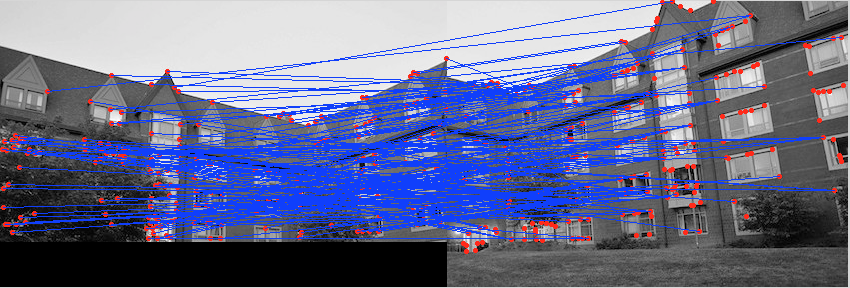
\includegraphics[width=0.9\linewidth]{../latex/allmatches.png} \\
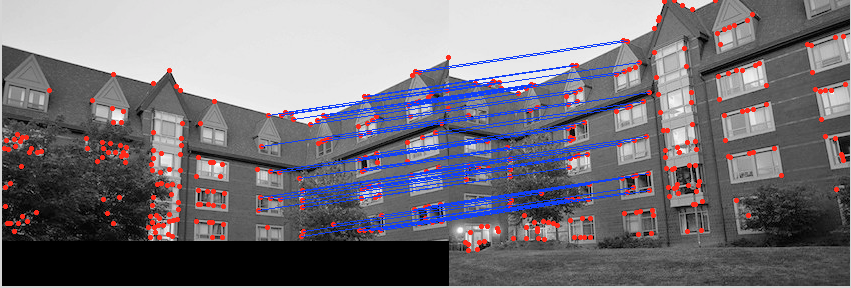
\includegraphics[width=0.9\linewidth]{../latex/inliers.png} \\
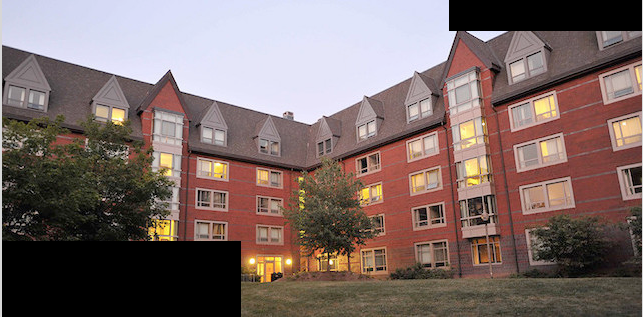
\includegraphics[width=0.9\linewidth]{../latex/result.png} \\
\end{figure}
\newpage

\item Outputs for \cmd{umass\_building\_right2.jpg}
\begin{figure}[h]
\centering
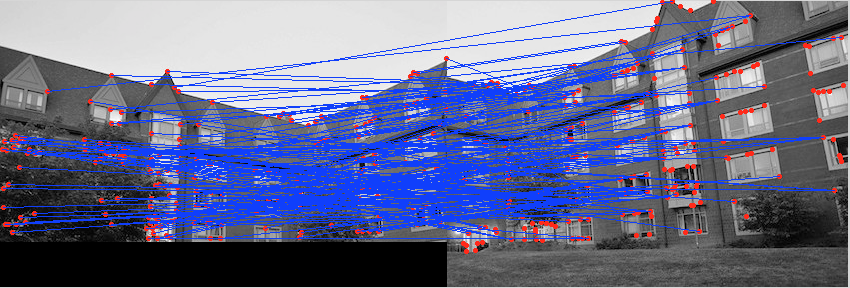
\includegraphics[width=0.9\linewidth]{../latex/allmatches.png} \\
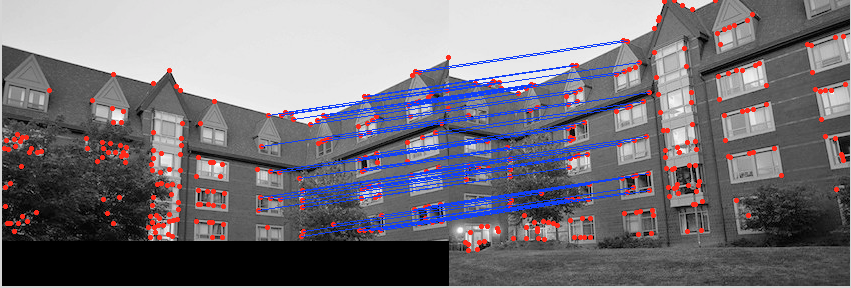
\includegraphics[width=0.9\linewidth]{../latex/inliers.png} \\
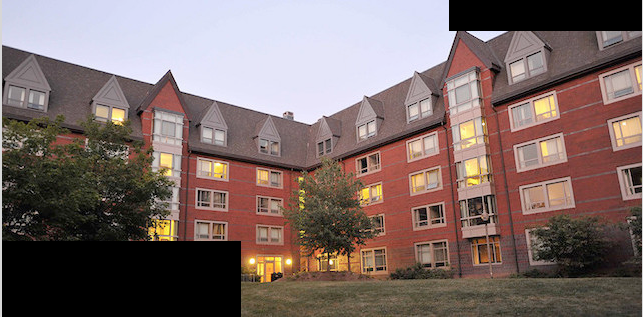
\includegraphics[width=0.9\linewidth]{../latex/result.png} \\
\end{figure}
\newpage

\item Outputs for \cmd{umass\_building\_right3.jpg}
\begin{figure}[h]
\centering
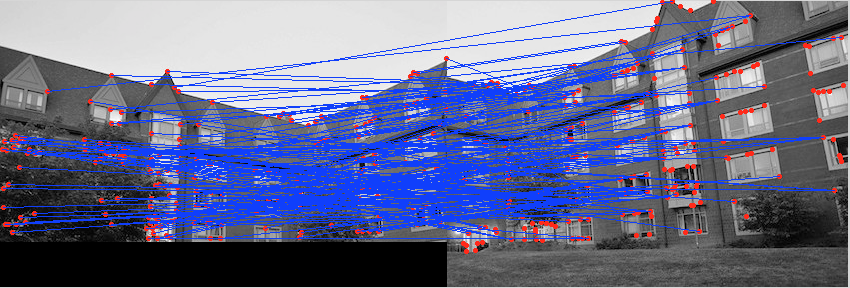
\includegraphics[width=0.9\linewidth]{../latex/allmatches.png} \\
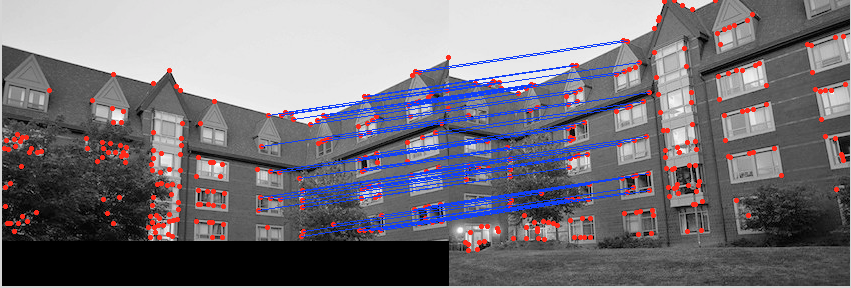
\includegraphics[width=0.9\linewidth]{../latex/inliers.png} \\
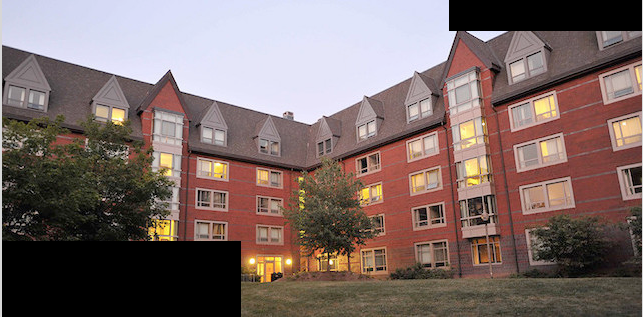
\includegraphics[width=0.9\linewidth]{../latex/result.png} \\
\end{figure}
\newpage

\item Outputs for \cmd{umass\_building\_right4.jpg}
\begin{figure}[h]
\centering
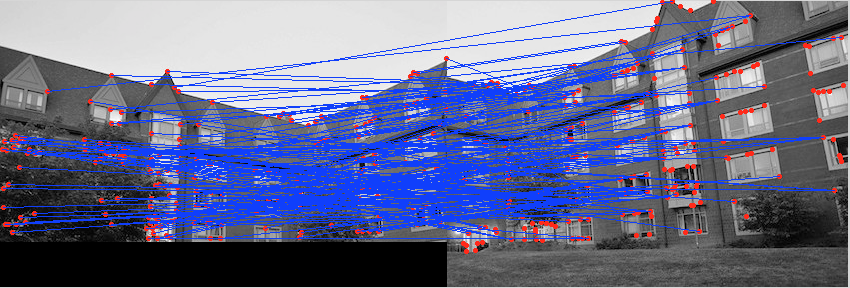
\includegraphics[width=0.9\linewidth]{../latex/allmatches.png} \\
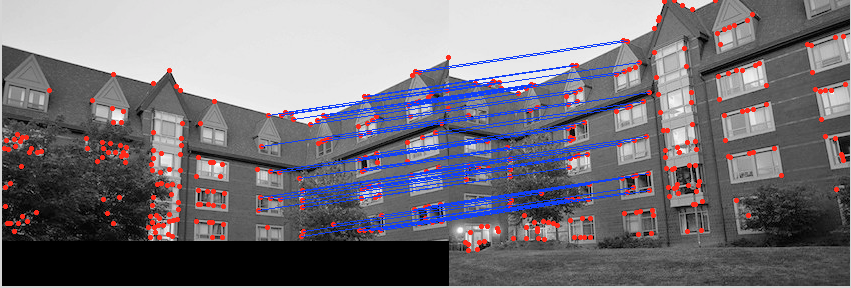
\includegraphics[width=0.9\linewidth]{../latex/inliers.png} \\
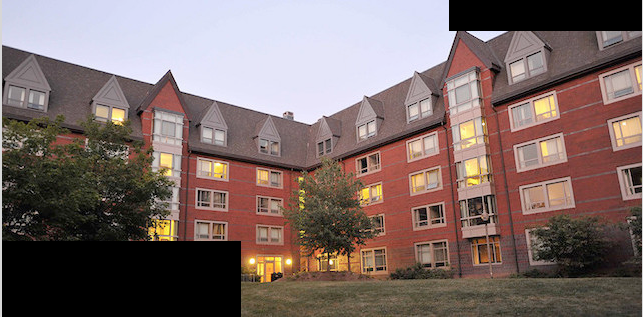
\includegraphics[width=0.9\linewidth]{../latex/result.png} \\
\end{figure}
\newpage

\item Outputs for \cmd{umass\_building\_right5.jpg}
\begin{figure}[h]
\centering
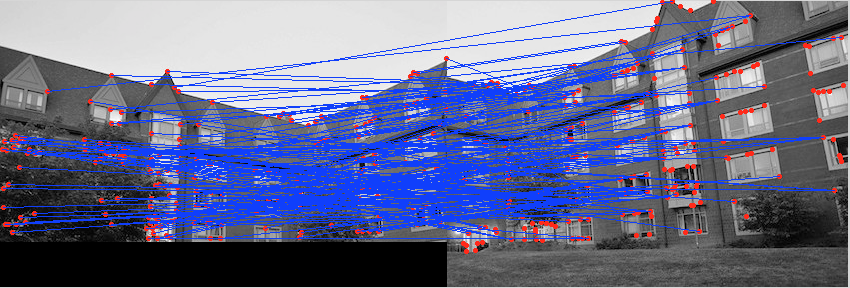
\includegraphics[width=0.9\linewidth]{../latex/allmatches.png} \\
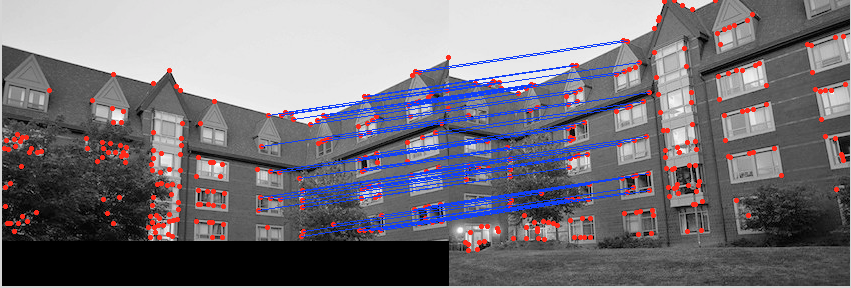
\includegraphics[width=0.9\linewidth]{../latex/inliers.png} \\
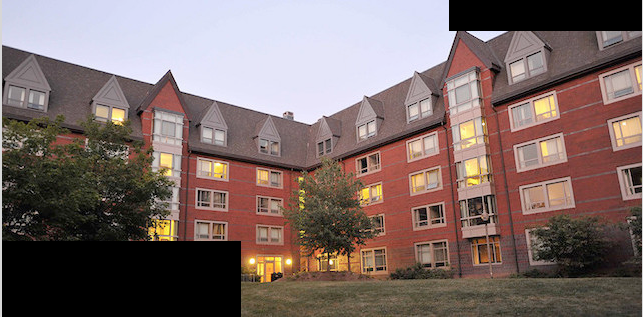
\includegraphics[width=0.9\linewidth]{../latex/result.png} \\
\end{figure}
\newpage

\item Estimated transformations and number of inliers
\begin{table}[h]
\centering
\begin{tabular}{c|c|c|c|c}
im2 & tx & ty & s & \#inliers\\
\hline
umass\_building\_right1.jpg & & & &\\
umass\_building\_right2.jpg & & & &\\
umass\_building\_right3.jpg & & & &\\
umass\_building\_right4.jpg & & & &\\
umass\_building\_right5.jpg & & & &\\
\end{tabular}
\caption{Estimated transformation.}
\end{table}

\end{itemize}


\section{Solution code}
Include the source code for your solutions as seen below (only the files you implemented are necessary). 
In latex the command \cmd{verbatiminput\{alignChannels.m\}} allows you to include the code verbatim as seen below. 
Regardless of how you do this the main requirement is that the included code is readable (use proper formatting, variable names, etc.)
A screenshot of your code works to provided you include a link to source files.



\subsection{extractFeatures.m}
\verbatiminput{../code/extractFeatures.m}
\subsection{computeMatches.m}
\verbatiminput{../code/computeMatches.m}
\subsection{ransac.m}
\verbatiminput{../code/ransac.m}
\end{document}
